\section{Results}   \label{sec:results}
% Results

%% Able to approximate the feasable control region by solving QP over large displacement space

%% Can do steady state control of 2dof system to within ____ m displacement and ____ degrees rotation

%% Plot comparing the the desired end effector positions to those achieved
\begin{figure}
    \centering
    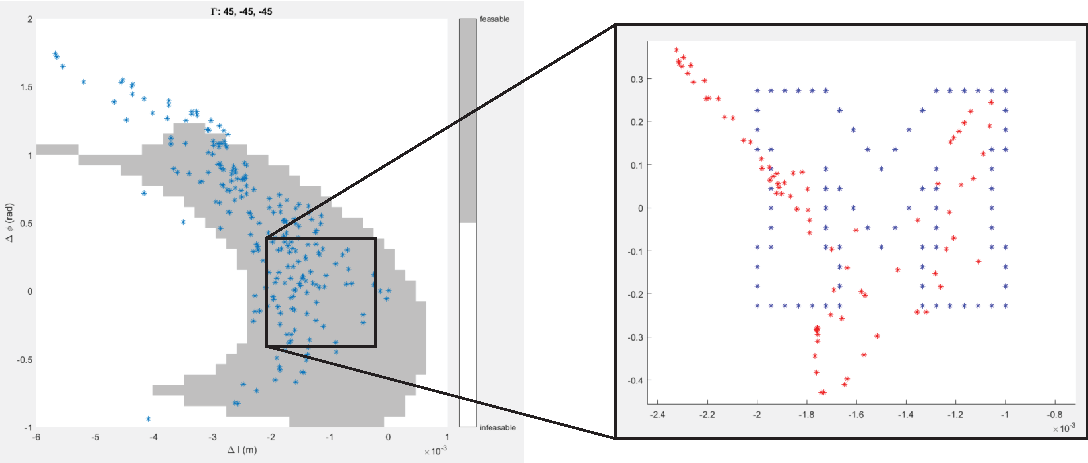
\includegraphics[width=\linewidth]{figures/resultsDiagram.pdf}
    \caption{(a) The feasable control region calculated by the model with measured test points over range of admissable pressures superimposed. (b) Desired end effector positions compared to measured end effector positions at corresponding pressures. \Dan{Placeholder figure and caption just to show the proposed structure. Didn't want to waste time nicely formatting bad results.}}
    \label{fig:results}
\end{figure}
